%
% hardware.tex
%
% Copyright (C) 2021 by SpaceLab.
%
% TTC Documentation
%
% This work is licensed under the Creative Commons Attribution-ShareAlike 4.0
% International License. To view a copy of this license,
% visit http://creativecommons.org/licenses/by-sa/4.0/.
%

%
% \brief Hardware description chapter.
%
% \author Gabriel Mariano Marcelino <gabriel.mm8@gmail.com>
%
% \institution Universidade Federal de Santa Catarina (UFSC)
%
% \version 1.2.0
%
% \date 2021/01/16
%

\chapter{Hardware} \label{ch:hardware}

The TTC board is composed by the following main components:

\begin{itemize}
	\item MSP430F6659, as the beacon microcontroller.
	\item RF4463F30, as the radio module for the beacon and the telemetry link.
\end{itemize}

In the figure \ref{fig:ttc-board}, ...

\begin{figure}[!h]
	\begin{center}
		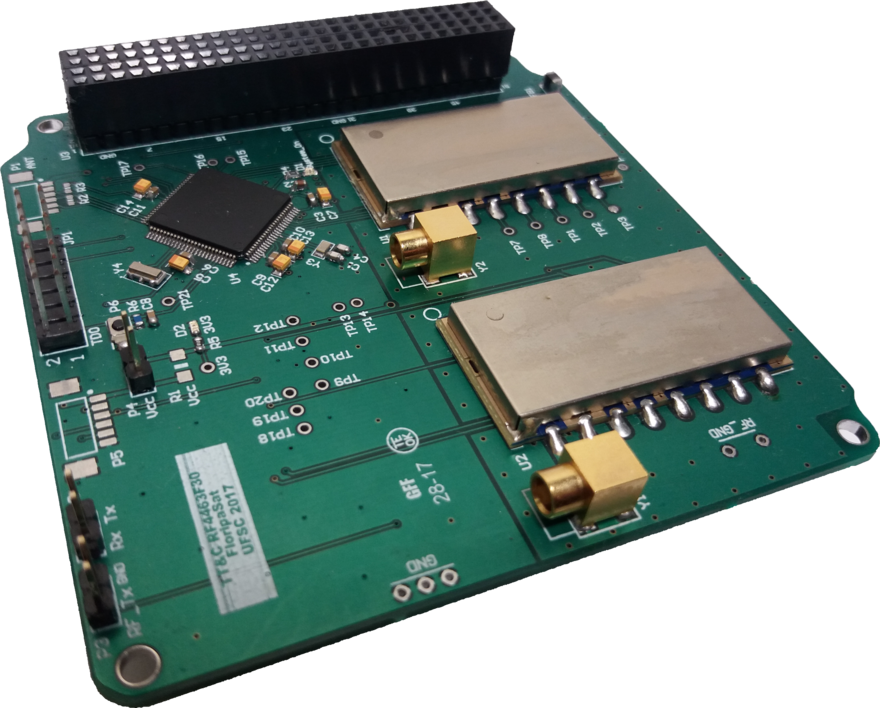
\includegraphics[width=0.75\textwidth]{figures/ttc_board.png}
		\caption{TTC PCB.}
		\label{fig:ttc-board}
	\end{center}
\end{figure}

\section{General Diagram}

In the figure \ref{fig:hardware-diagram}, a general hardware diagram can be seen, with the connection and protocols between the components.

\begin{figure}[!h]
	\begin{center}
		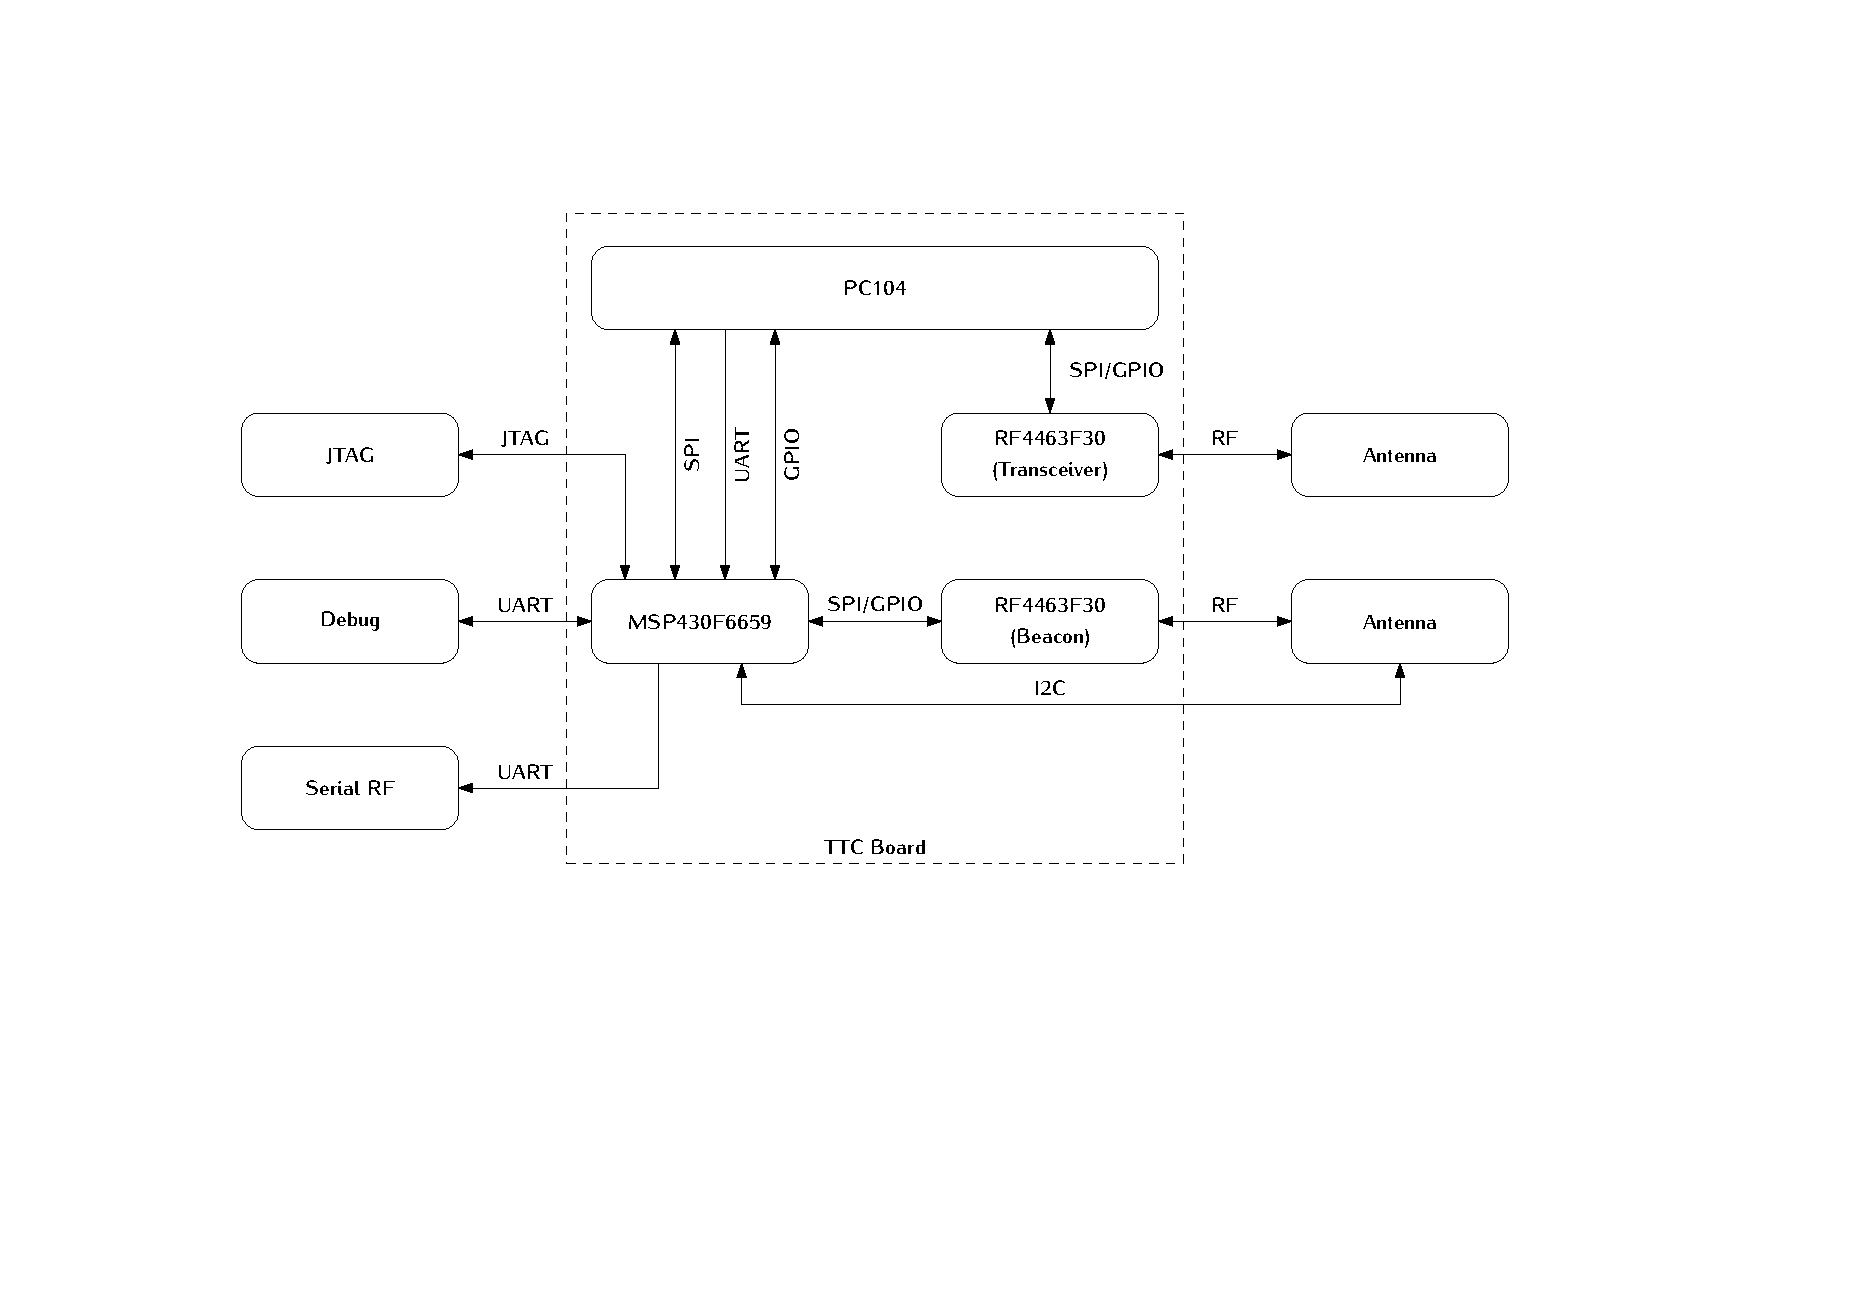
\includegraphics[width=\textwidth]{figures/hardware_diagram.pdf}
		\caption{Hardware diagram of the TTC module.}
		\label{fig:hardware-diagram}
	\end{center}
\end{figure}

\section{Main Components}

\subsection{Microcontroller}

The beacon microcontroller is the MSP430F6659IPZR \cite{msp430f6659}. Its main characteristics can be found in the table \ref{tab:msp430f6659-info}.

\nomenclature{\textbf{CPU}}{Central Processing Unit.}
\nomenclature{\textbf{RAM}}{Random Access Memory.}
\nomenclature{\textbf{GPIO}}{General Purpose Input/Output.}
\nomenclature{\textbf{I$^{2}$C}}{Inter-Integrated Circuit.}
\nomenclature{\textbf{SPI}}{Serial Peripheral Interface.}
\nomenclature{\textbf{UART}}{Universal Asynchronous Receiver/Transmitter.}
\nomenclature{\textbf{DMA}}{Direct Memory Access.}
\nomenclature{\textbf{ADC}}{Analog-To-Digital Converter.}
\nomenclature{\textbf{BSL}}{Bootstrap Loader.}

\begin{table}[!h]
	\begin{center}
		\begin{tabular}{lc}
			\toprule[1.5pt]
			\textit{Characteristic} & \textit{Value} \\
			\midrule
			CPU & MSP430 \\
			Frequency & Up to 20 MHz \\
			Non-volatile memory & 512 kB \\
			RAM & 66 kB \\
			GPIO pins & 74 \\
			I$^{2}$C & 3 \\
			SPI & 6 \\
			UART & 3 \\
			DMA & 6 \\
			ADC & ADC12-12ch \\
			Comparators & 12 inputs \\
			Timers - 16-bit & 4 \\
			Multiplier & $32 \times 32$ \\
			BSL & USB \\
			Min $V_{cc}$ & 1,8 V \\
			Max $V_{cc}$ & 3,6 V \\
			Active Power & $360\ \mu A/MHz$ \\
			Standby Power (LMP3) & $2,6\ \mu A$ \\
			Wakeup Time & $3\ \mu s$ \\
			Operating Temperature Range & -40 to 80 $^{\circ}C$ \\
			\bottomrule[1.5pt]
		\end{tabular}
		\caption{MSP430F6659 features.}
		\label{tab:msp430f6659-info}
	\end{center}
\end{table}

\subsection{Radio Modules}

The NiceRF RF4463F30 \cite{rf4463f30} is a transceiver module based on the Silicon Labs Si4463 \cite{si4463} radio. This module also contains a PA module to increase the output power up to 31 dBm.

In compliance with the \textit{TMR 3}, the RF4463F30 module operates with 5 V as input voltage in the TTC board, to achieve 30 dBm (1 W) in its output (The RF connector).

\subsubsection{Si4463}

The RF4463F30 module uses the Si4463 radio module. The main characteristics of this IC can be found in the table \ref{tab:si4463-info}.

\begin{table}[!h]
	\begin{center}
		\begin{tabular}{lcc}
			\toprule[1.5pt]
			\textit{Characteristic} & \textit{Value} & \textit{Unit} \\
			\midrule
			Frequency range & 119-1050 & MHz \\
			Receiver sensitivity & -126 & dBm \\
			Modulation & (G)FSK, 4(G)FSK, (G)MSK and OOK & - \\
			Max. output power & +20 & dBm \\
			PA support & +27 to 30 & dBm \\
			Ultra low current powerdown modes & 30 (shutdown), 50 (standby) & nA \\
			Data rate & 100 bps to 1 Mbps & - \\
			Power supply & 1,8 to 3,6 & V \\
			TX and RX FIFOs & 64 bytes for each or 129 bytes shared & - \\
			\bottomrule[1.5pt]
		\end{tabular}
		\caption{Si4463 features.}
		\label{tab:si4463-info}
	\end{center}
\end{table}

\section{External Connections}

This section describes the external available connections of the TTC module.

In the figure \ref{fig:connections-ref}, all the external connections are enumerated.

\begin{figure}[!h]
	\begin{center}
		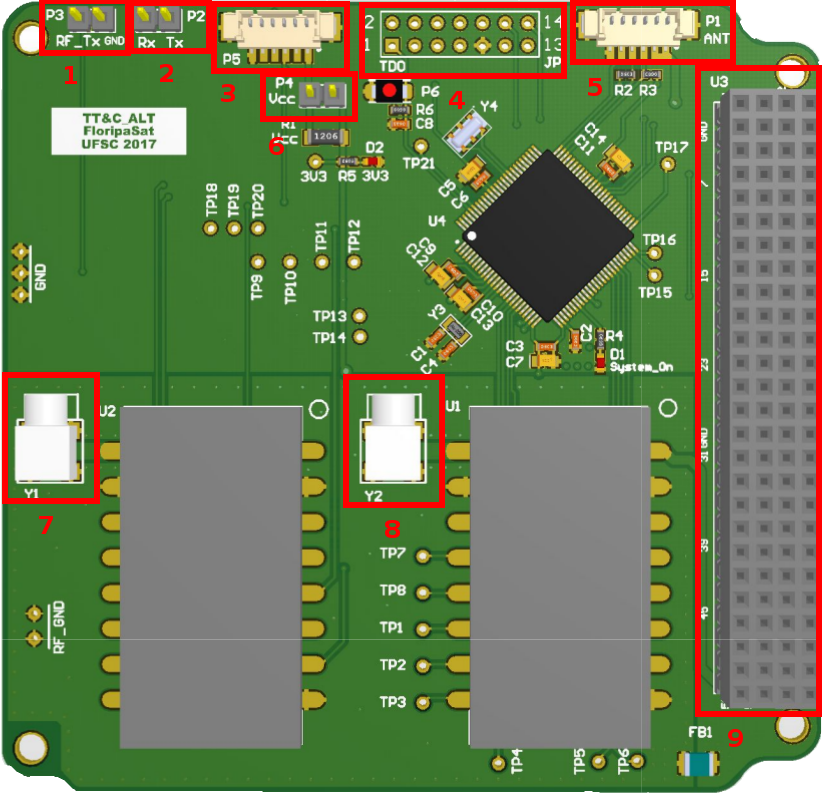
\includegraphics[width=0.75\textwidth]{figures/ttc_board_pins}
		\caption{External connections on the board.}
		\label{fig:connections-ref}
	\end{center}
\end{figure}

A brief description of each connection is presented in the table \ref{tab:connections-ref}.

\begin{table}[!h]
	\begin{center}
		\begin{tabular}{L{1.3cm} C{3cm} C{10cm}}
			\toprule[1.5pt]
			\textit{Number} & \textit{Connector} & \textit{Description} \\
			\midrule
			1 & Male pin header ($1 \times 2$) & UART TX $@$4800 bps. These pins transmit the beacon packets over a serial connection (It is enable in the configuration file, setting the BEACON\_RADIO variable as UART\_SIM). \\
			2 & Male pin header ($1 \times 2$) & Debug UART TX/RX $@$115200 bps. These pins transmit a description of the main events of the beacon software during it's execution. This feature is only available in DEBUG\_MODE. \\
			3 & Male PicoBlade$^{TM}$ ($\times 6$) & JTAG and Debug. This connection contains the relevant pins of the connectors 2 and 4. \\
			4 & Male pin header ($2 \times 2$) & MSP430 JTAG. This connection is for programming the uC code, using a MSP-FET debugger. \\
			5 & Male PicoBlade$^{TM}$ ($\times 6$) & Antenna I2C. I2C bus for a communication channel with the antenna module. \\
			6 & Male pin header ($1 \times 2$) & Power supply jumper. With a jumper, the beacon microcontroller power source comes from the JTAG connector. Without a jumper, the uC power supply comes from a pin of the PC104 connector. \\
			7 & Female Angled MCX & 437 MHz band RF signal (Goes to the antenna module). \\
			8 & Female Angled MCX & 145 MHz band RF signal (Goes to the antenna module). \\
			9 & Male/Female PCI-104 & PCI-104. Power supply and communication buses with others stacked up modules. \\
			\bottomrule[1.5pt]
		\end{tabular}
		\caption{External connections description.}
		\label{tab:connections-ref}
	\end{center}
\end{table}

The connections 1, 2, 4 and 6 were designed to be used during the software development stage, and not during the satellite operation.

\subsection{PCI-104 Pins}

The table \ref{tab:pci104-ref} describes the PCI-104 connector used pins. The first column is the row number of the connector, and the remaining columns are the respective columns (Named as H1A, H1B, H2A and H2B respectively). If the pin has no description, it is not connected to the TTC board.

\begin{table}[!h]
	\begin{center}
		\begin{tabular}{L{1cm} C{3cm} C{3cm} C{3cm} C{3cm}}
			\toprule[1.5pt]
			\textit{Row} & \textit{H1A} & \textit{H1B} & \textit{H2A} & \textit{H2B} \\
			\midrule
			1 & GND & GND & GND & GND \\
			2 & GND & GND & GND & GND \\
			3 & - & - & UART RX $@$4800 bps from the EPS module. & - \\
			4 & Telemetry radio GPIO0 & Telemetry radio GPIO1 & - & - \\
			5 & Telemetry radio GPIO2 & Enable beacon radio power supply & - & - \\
			6 & Telemetry radio SDN & - & OBDH communication (SPI MOSI) & OBDH communication (SPI clock) \\
			7 & - & - & OBDH communication (SPI chip select) & OBDH communication (SPI MISO) \\
			8 & - & - & - & - \\
			9 & - & - & - & - \\
			10 & - & - & - & - \\
			11 & - & - & - & - \\
			12 & - & - & - & - \\
			13 & - & - & - & - \\
			14 & - & - & Beacon uC power supply (3,3 V/50 mA) & 3,3 V beacon uC power supply (3,3 V/50 mA) \\
			15 & GND & GND & GND & GND \\
			16 & GND & GND & GND & GND \\
			17 & - & - & - & - \\
			18 & Telemetry radio SPI clock & - & - & - \\
			19 & Telemetry radio SPI MISO & - & - & - \\
			20 & Telemetry radio SPI MOSI & Telemetry radio SPI chip select & - & - \\
			21 & - & - & - & - \\
			22 & - & - & - & - \\
			23 & - & - & - & - \\
			24 & - & - & - & - \\
			25 & Telemetry radio power supply (5 V/500 mA) & - & - & - \\
			26 & Beacon radio power supply (5 V/500 mA) & - & - & - \\
			\bottomrule[1.5pt]
		\end{tabular}
		\caption{PCI-104 connector reference.}
		\label{tab:pci104-ref}
	\end{center}
\end{table}

\section{PCB}

The PCB (Printed Circuit Board) of the TTC module has basically the MSP430F6659 ic, the RF4463F30 module and all the external connectors.

Some characteristics of this PCB are described bellow:

\begin{itemize}
	\item The components and traces of the board are distributed over two layers (one in each side of the board).
	\item The RF modules are placed in a isolated ground plane (Connected to the main GND using a ferrite bead). This region can be seen in the figure \ref{fig:rf-ground-plane}.
	\item The antenna output of the RF4463F30 modules are connected to their respective connector over a 50 Ohm coupled trace.
\end{itemize}

\begin{figure}[!h]
	\begin{center}
		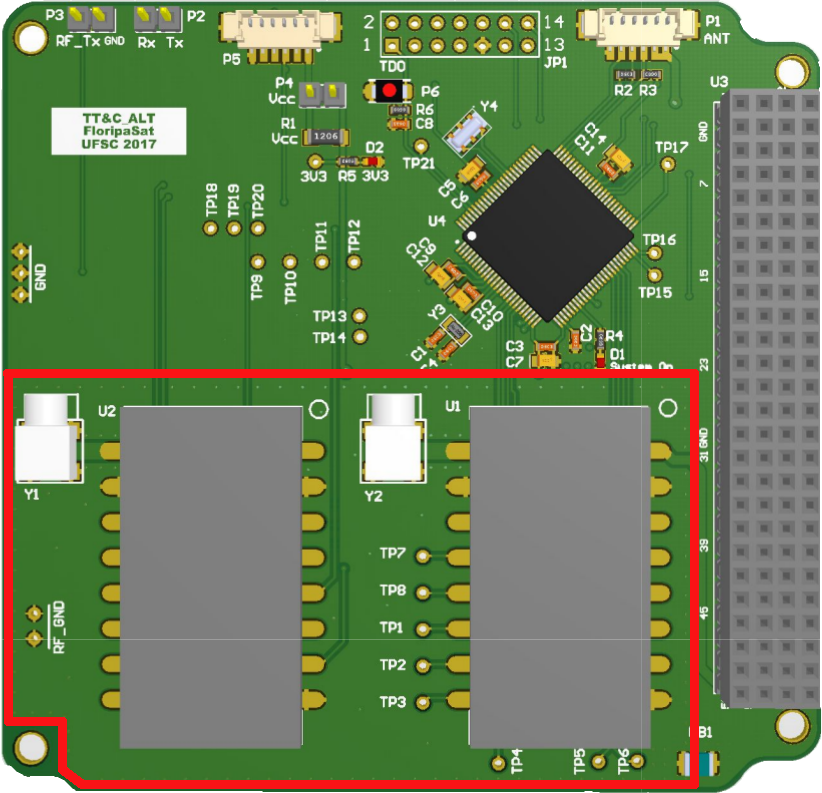
\includegraphics[width=0.5\textwidth]{figures/ttc_rf_ground_plane.png}
		\caption{RF ground plane region (red) of the TTC board.}
		\label{fig:rf-ground-plane}
	\end{center}
\end{figure}

\subsection{Types of assembly}

The TTC PCB has two types of assembly: Develop and flight.

The develop type has the purpose to be used during the development stage and tests. In this version, the connectors 3 and 5 are not soldered (Using the figure \ref{tab:connections-ref} as reference).

The flight version were designed to be used during the satellite operation. In this version, the connectors 1, 2, 4 and 6, and the reset button, are not soldered.

\section{Power Budget}

\begin{figure}[!h]
	\begin{center}
		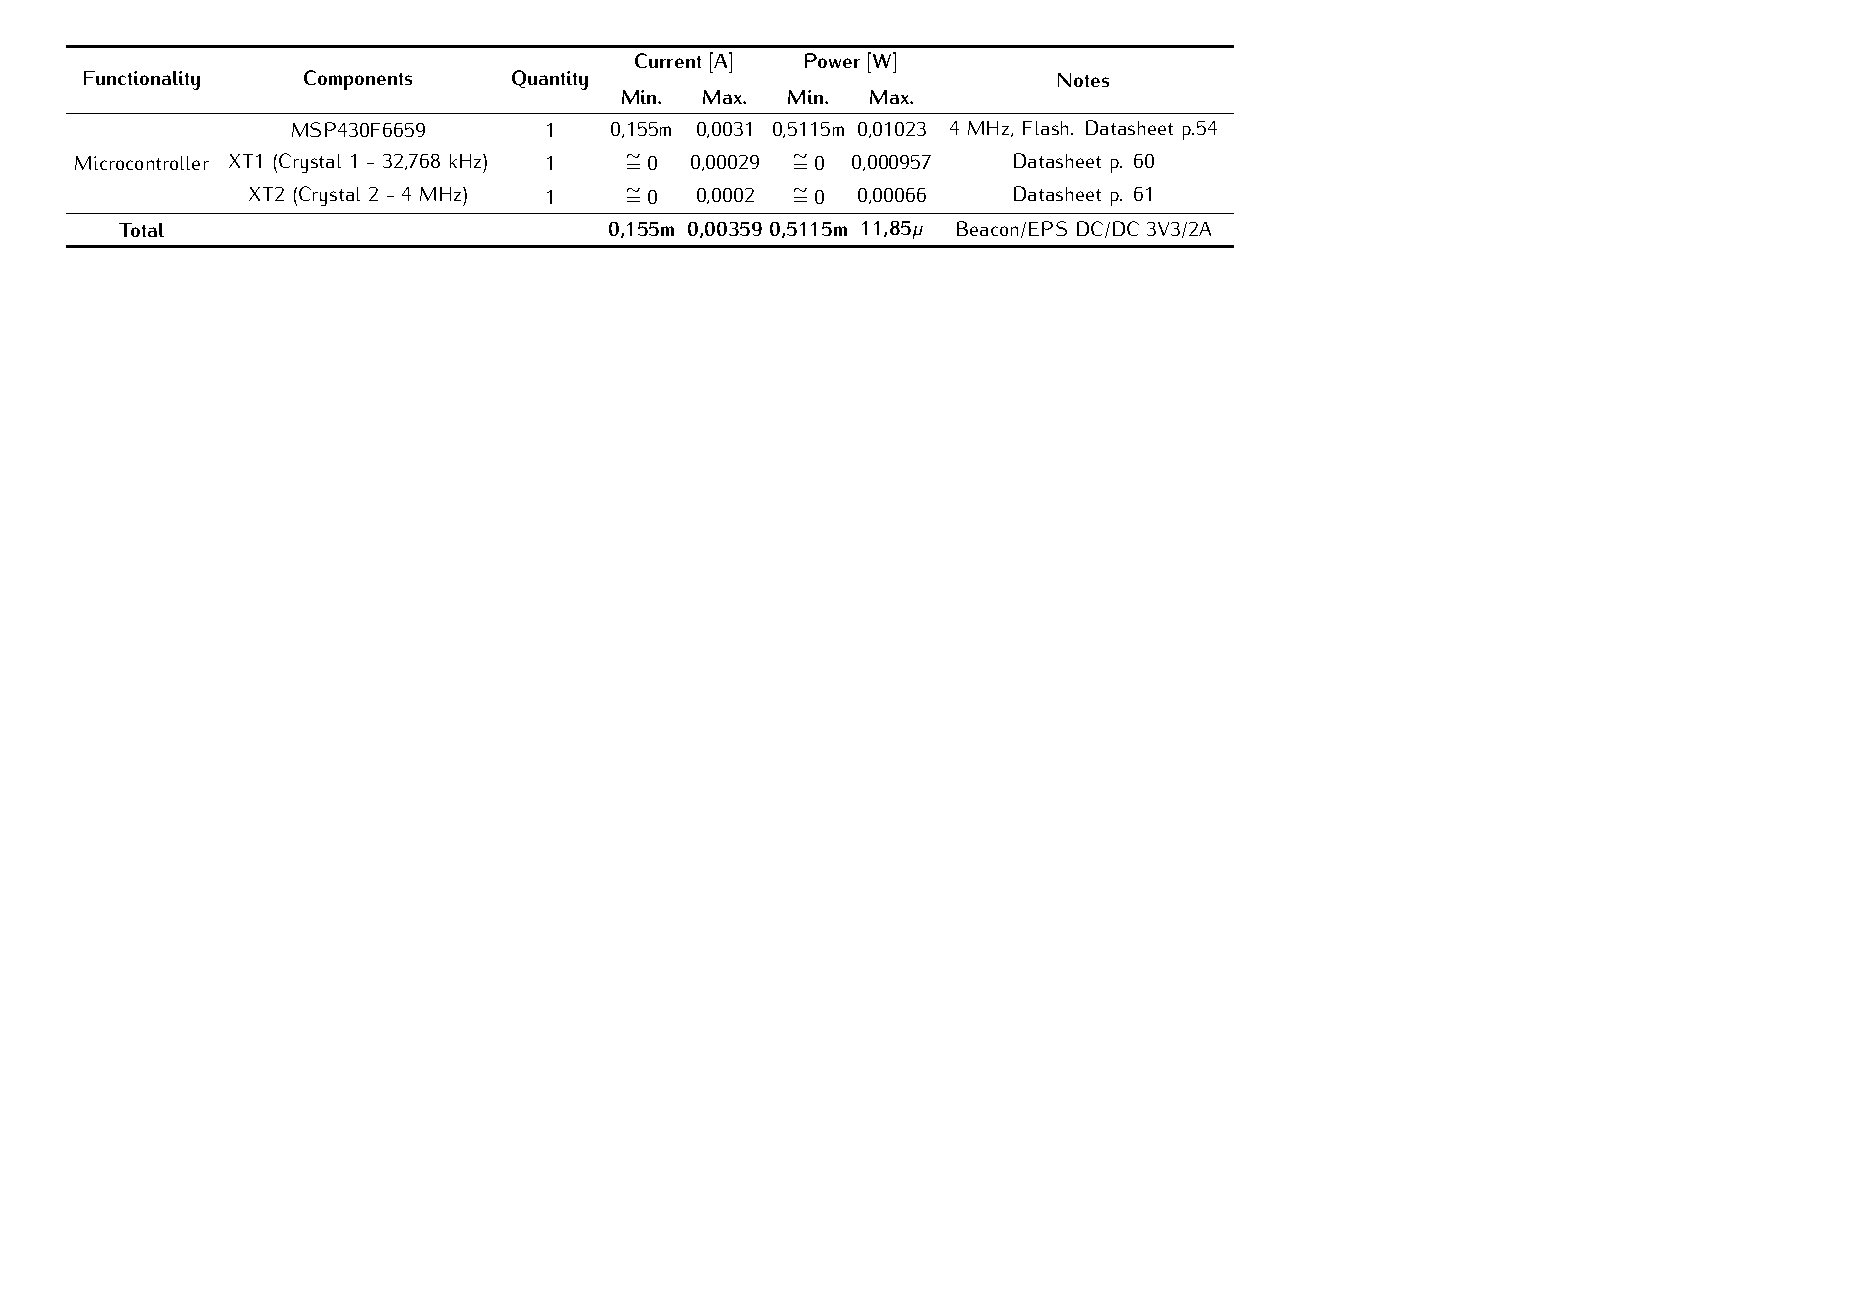
\includegraphics[width=\textwidth]{figures/power_budget_static.pdf}
		\caption{Static power budget of the TTC module.}
		\label{fig:power-budget-static}
	\end{center}
\end{figure}

\begin{figure}[!h]
	\begin{center}
		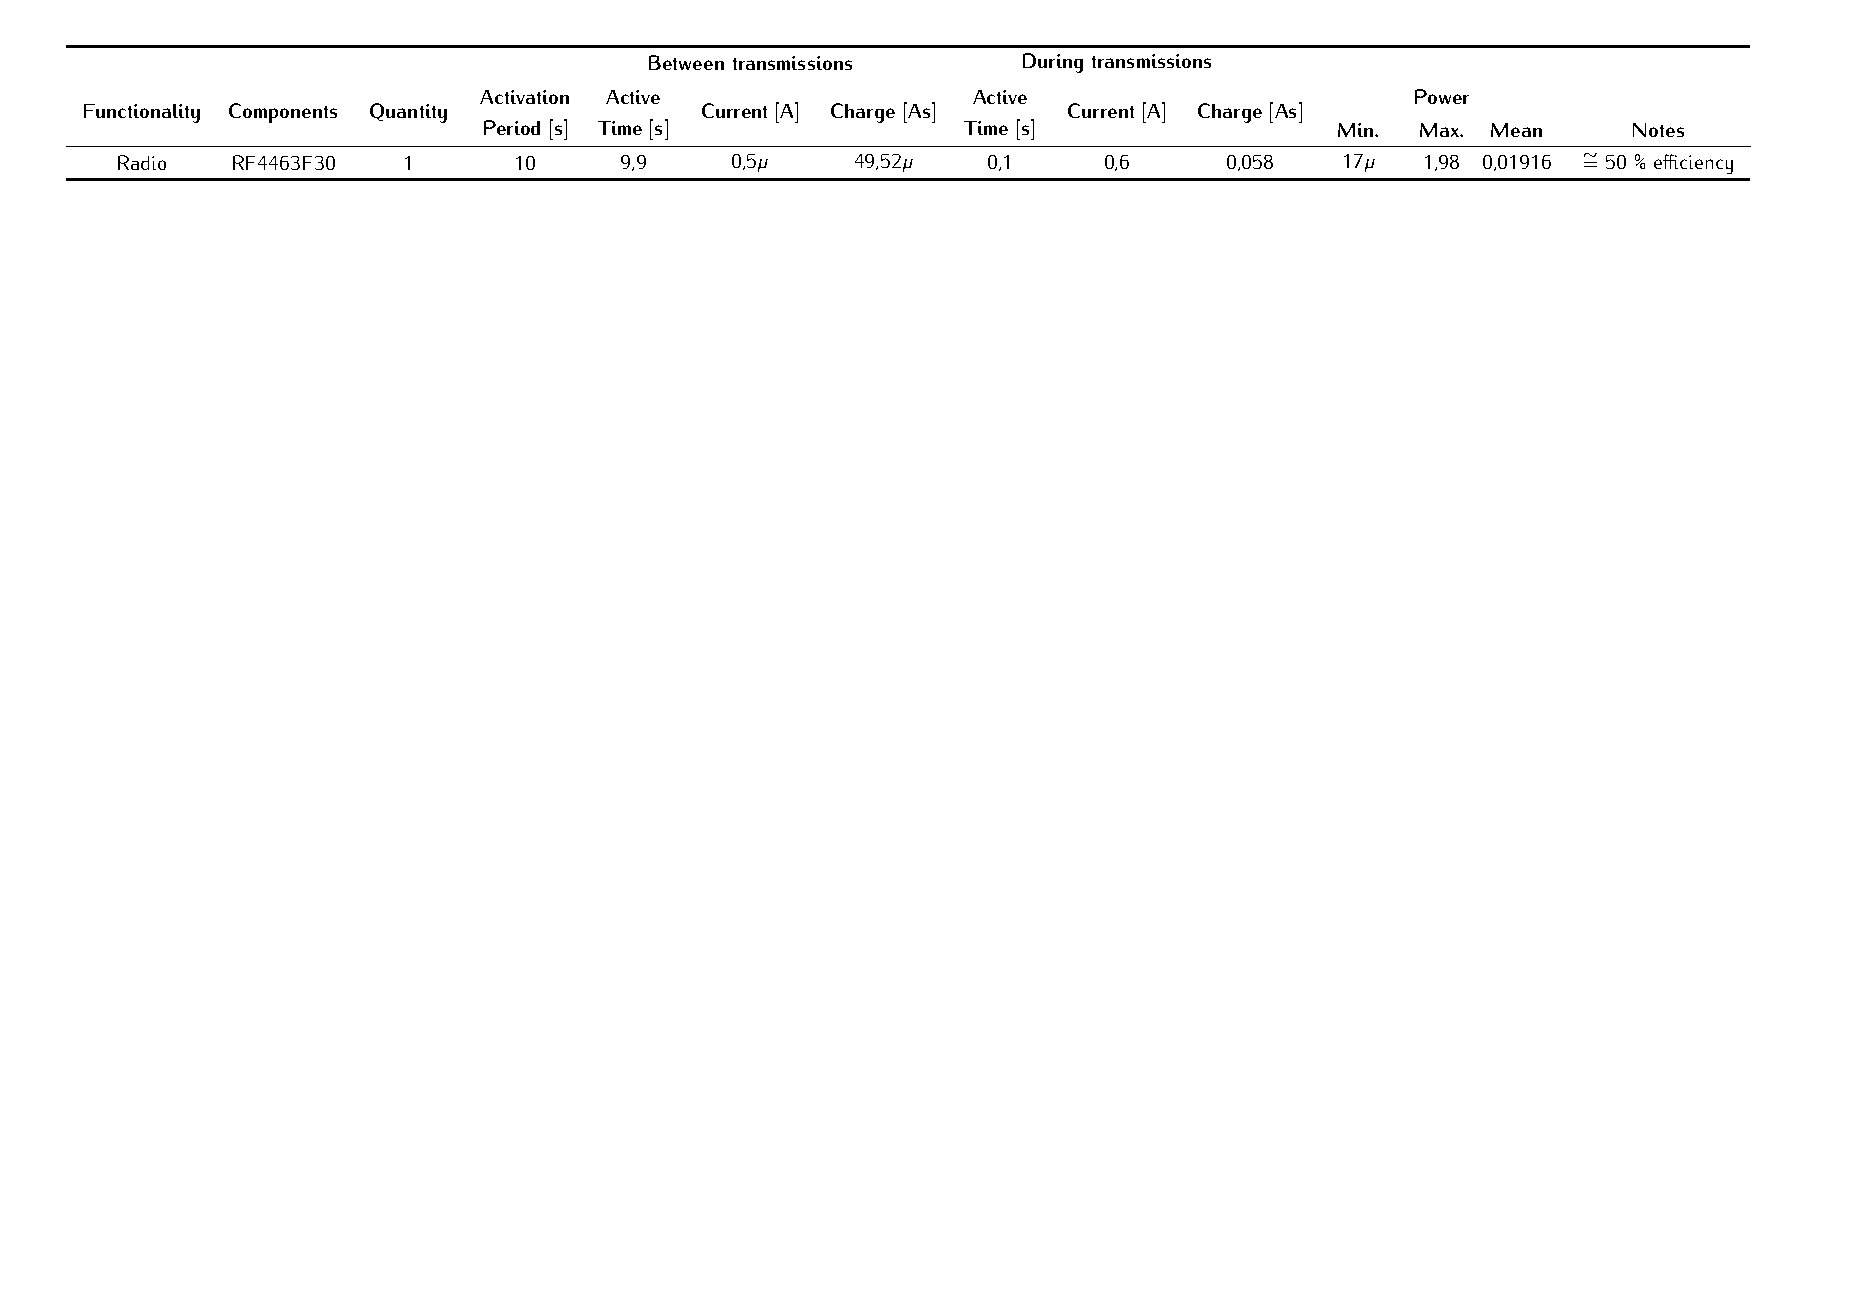
\includegraphics[width=\textwidth]{figures/power_budget_dynamic.pdf}
		\caption{Dynamic power budget of the TTC module.}
		\label{fig:power-budget-dynamic}
	\end{center}
\end{figure}
